\documentclass{beamer}
\usepackage{HECbeamer}
% \usepackage{pgfpages}
% \pgfpagesuselayout{4 on 1}[letterpaper, landscape, border shrink=5mm]
\title[\color{white}{MATH 60604 \S~7a - Concepts d'analyse de survie}]{\texorpdfstring{MATH 60604 \\Modélisation statistique \\ \S~7a - Concepts d'analyse de survie}{MATH 60604 \\ Modélisation statistique \\ \S~7a - Concepts d'analyse de survie}}
\author{Léo Belzile}
\institute{HEC Montréal\\
Département de sciences de la décision}
\date{} 

\begin{document}
\frame{\titlepage}
\begin{frame}
\frametitle{Données de survie}
\begin{itemize}
\vp \vp
\item Dans le cadre de \alert{l'analyse de survie}, on s'intéresse au temps jusqu'à ce qu'un événement survienne, une variable réponse positive.
\item Soit $T_i$ le \alert{temps de survie} pour le sujet $i$ ($i=1, \ldots, n$). 
\item Le temps de survie avant que l'événement d'intérêt survienne. 
\begin{itemize}
\vp \vp
\item Généralement continue, mais mesurée à des moments précis (données discrètes).
\item Le temps de survie est aussi appelé \alert{temps de défaillance}.
\end{itemize}
\item Les données de survie sont particulières et il est essentiel d'avoir une bonne compréhension des méchanismes générateurs des données afin d'effectuer une analyse appropriée. 
\end{itemize}
\end{frame}
\begin{frame}
\frametitle{Exemples de données de survie}
Parmi les exemples, 
\begin{itemize}
\vp \vp
\item le temps avant le décès d'un patient à qui on a diagnostiqué un cancer 
\item le temps avant qu'un hôpital donne congé à un patient 
\item le temps d'attente avant qu'un client soit servi dans un restaurant
\item le temps précédant l'annulation d'un abonnement à un gym
\item le temps avant qu'une ampoule brûle
\end{itemize}
\end{frame}
% \begin{frame}
% \frametitle{Temps d'entrée}
% Afin de pouvoir bien définir le temps de survie $T_i$, il faut avoir une notion du \alert{temps d'entrée}, ou le temps de départ, pour le sujet $i$. 
% \begin{itemize}
% \vp \vp
% \item C'est-à-dire, le temps auquel $T_i=0$, quand nous démarrons le chronomètre.
% \end{itemize}
% Le temps d'entrée dépend du contexte de l'étude. 
% \begin{itemize}
% \vp \vp
% \item Le temps d'entrée peut être le même pour tous les sujets. 
% \begin{itemize} \item le temps que ça prend une cohorte d'étudiants pour compléter leurs études
% \end{itemize} 
% % , et que tous ces étudiants commencent à l'automne 2019.
% \item Le temps d'entrée peut être différent d'un sujet à un autre. 
% \begin{itemize} \item le temps avant qu'un client qui attend en ligne soit servi. 
% \end{itemize} 
% \end{itemize}
% % \end{itemize}
% \end{frame}

\begin{frame}
\frametitle{Censure}
\begin{itemize}
 \item La variable d'intérêt est le temps $T_i$ avant que l'événement survienne.
% \item Cependant, au cours de la période d'étude, l'événement ne survient pas nécessairement pour chaque sujet.
\item Une des plus grandes difficultés avec l'analyse de survie est qu'\textbf{on n'observe pas nécessairement tous les événements}.
\item Cela pourrait être parce que
\begin{itemize}
\vp \vp
\item le sujet survit après la fin de la période d'étude,
\item le sujet quitte l'étude avant la fin,
\item un autre événement se produit, ce qui rend l'événement d'intérêt impossible.
\end{itemize}
\end{itemize}
\end{frame}
% 
% \begin{frame}
% 
% \item Cela est appelée la \alert{censure}.
% \begin{itemize}
% \vp \vp
% \item Quand un observation est censurée, c'est comme si nous avons que de l'information partielle sur le sujet.
% \end{itemize}
% \end{itemize}
% \end{frame}


\begin{frame}
\frametitle{Exemples de censure à droite}
 Le type de censure le plus commun est la \alert{censure à droite}: on sait juste que l'événement se produit après un certain temps $t$, c'est-à-dire $T_i \geq t$.

\begin{itemize}
\vp \vp
\item $T$ représente le temps de survie d'un individu après avoir été diagnostiqué avec un cancer
\begin{itemize} \item il se peut que le sujet soit toujours vivant à la fin de l'étude.
\end{itemize}
\item $T$ représente le temps que ça prend à un étudiant pour compléter leur programme 
\begin{itemize} \item
il se peut que certains étudiants abandonnent leur programme.
\end{itemize}
\item $T$ représente le nombre d'années de service avant la retraite pour des employées d'un entreprise 
\begin{itemize} \item il se peut qu'un sujet décède avant de prendre sa retraite. 
\end{itemize}
\end{itemize}

\end{frame}


\begin{frame}
\frametitle{Types de censure}
\begin{itemize}
\item Il existe d'autres types de censure aussi:
\begin{itemize}
\vp \vp
\item \textbf{censure à gauche}: l'événement d'intérêt survient avant qu'on observe l'individu. C'est-à-dire, tout ce qu'on sait est que $T<t$.
\item \textbf{censure par intervalle}: l'événement d'intérêt survient à un point inconnu dans un intervalle de temps, mais on ne sait pas quand exactement. C'est-à-dire, tout ce qu'on sait est que $T \in [t_1,t_2]$
\end{itemize}
\item On va se concentrer sur la censure à droite. 
\item Avec la censure, l'idée générale est qu'on ne sait la valeur précise de $T$, mais on a tout de même de l'information concernant un intervalle dans laquelle $T$ peut tomber.
\begin{itemize}
\vp \vp
\item par ex: $T>t$, ou $T<t$, ou $T \in [t_1,t_2]$
\end{itemize}
\end{itemize}
\end{frame}

\begin{frame}
\frametitle{Examples de censure}
\begin{itemize} \item Supposons qu'un chercheur s'intéresse à l'âge à partir duquel les enfants sont capables d'écrire leur prénom. 
\item $T$ est le temps (en années) jusqu'à ce qu'un enfant puisse écrire son nom. 
\item Le chercheur suit un groupe d'enfants dans une classe de maternelle tout au long de l'année scolaire. 
\begin{itemize} \item Lorsque le chercheur arrive, certains enfants sont déjà capables d'écrire leur nom: $T$ est \emph{censuré à gauche}. 
\item Certains enfants apprennent à écrire leur prénom pendant les vacances de Noël: $T$ est \emph{censuré par intervalle}. \item Certains enfants ne savent toujours pas comment écrire leur nom rendu à la fin de l'année scolaire:  $T$ est \emph{censuré à droite}.
\end{itemize}
\end{itemize}
\end{frame}


\begin{frame}
\frametitle{Censure non-informative}
\begin{itemize}
\item Nous supposons généralement que la censure est \alert{non-informative}. 
\begin{itemize}
\vp \vp
\item C'est-à-dire, la censure est non-informative de l'événement; le temps de censure est indépendant du temps de survie.
\item Autrement dit, le temps de censure ne nous donne aucune information sur ce que pourrait être le temps de survie.
\end{itemize}
\item Un exemple de censure \emph{informative}:
\begin{itemize}
\vp \vp
\item Supposons qu'un groupe de patients en phase terminale d'une maladie suit un traitement expérimental, et que ce traitement peut avoir des effets secondaires nocifs. Donc, pour des raisons éthiques, les patients qui deviennent très malades sont retirés de l'étude. Les patients qui sont retirés de l'étude auront un temps $T$ qui est censuré à droite. Cependant, ces patients qui abandonnent l'étude sont probablement en moins bonne santé et risquent davantage de mourir plus tôt.
\end{itemize}
\end{itemize}
\end{frame}
\begin{frame}
\frametitle{Type de censure à droite non-informative}
 On distingue entre plusieurs formes de censure à droite qui est non-informative:
 \begin{itemize} \item censure de type 1: la collecte de donnée prend fin au temps $C$; toute observation résiduelle est censurée à droite.
 \item censure de type 2: on collecte des données jusqu'à un nombre prédéterminé $k$ d'événements.
 \item \textbf{censure aléatoire}: le temps de survie observé est $T_i = \min\{T_i^0, C_i\}$, où la durée de survie $T_i^0$ et le temps de censure $C_i$ sont des variables aléatoires \textbf{indépendantes}. 
 \end{itemize}

\end{frame}

\begin{frame}
 \frametitle{Troncation}
 Dans certaines études, on collecte les données seulement pendant un créneau prédéterminé $[a, b]$. 
 \bi \item La trajectoire du temps est \textbf{tronquée à gauche} si le temps de survie excède zéro au temps $a$
\ei
Par exemple, lors d'une enquête sur le chômage, on considère toutes les personnes qui sont inscrites au chômage entre janvier et mars. 
\bi \item Certaines personnes ont perdu leur emploi depuis plusieurs mois lors du début de l'enquête (troncation à gauche). 
 \item Si la personne est toujours en recherche d'emploi à $b$, elle sera censurée à droite (censure à droite de type 1).
\ei
\end{frame}

\begin{frame}
\frametitle{Diagramme de Lexis}
 \begin{center}
  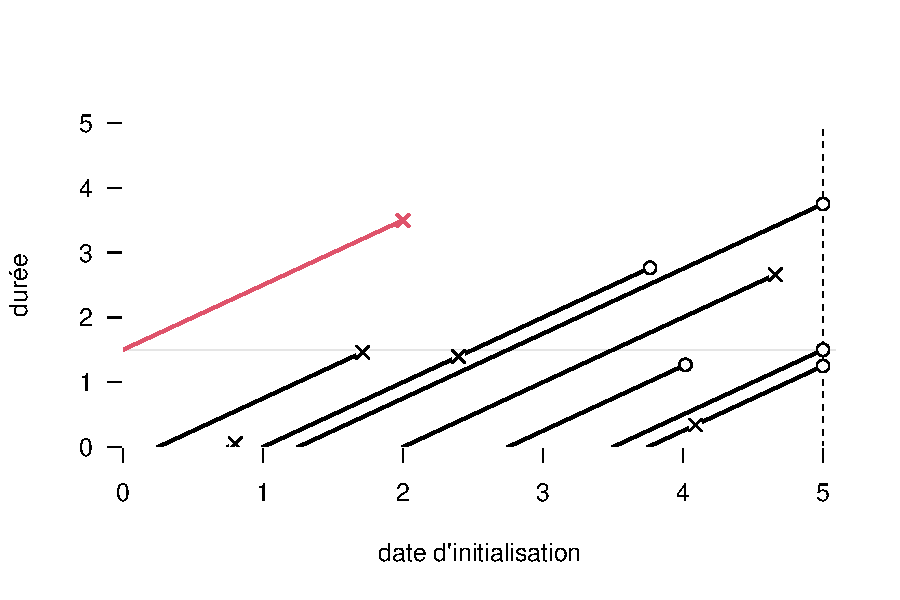
\includegraphics[width = 0.8\textwidth]{img/c7/07-lexis_fr.pdf}
 \end{center}
{ \footnotesize Diagramme de Lexis représentant les trajectoires temporelles. Les $\mathrm{x}$ dénotent les temps de défaillance observés, tandis que les $\circ$ indiquent les valeurs censurées. Les temps de survie résiduels au temps $5$ sont censurés. La trajectoire en rouge dénote un individu dont le temps de survie est tronqué à gauche.

}
\end{frame}
\end{document}
